%!TEX root = ../thesis_a4.tex

\chapter{Artist Similarity}
\label{sec:similarity}

\section{Introduction}\label{sec:introduction} %Todos

Artist biographies are a big source of musical context information and have been previously used for computing artist similarity. However, only shallow approaches have been applied by computing word co--occurrences and thus the semantics implicit in text have been barely exploited. To do so, semantic technologies, and more specifically Entity Linking tools may play a key role to annotate unstructured texts. These are able to identify named entities in text and disambiguate them with their corresponding entry in a knowledge base (e.g. Wikipedia, DBpedia or BabelNet).

This paper describes a method for computing semantic similarity at document-level, and presents evaluation results in the task of artist similarity. The cornerstone of this work is the intuition that semantifying and formalizing relations between entity mentions in documents (both at in-document and cross-document levels) can represent the relatedness of two documents. Specifically, in the task of artist similarity, this derives in a measure to quantify the degree of relatedness between two artists by looking at their biographies.

Our experiments start with a preprocessing step which involve Entity Linking over artist biographical texts. %using Babelfy \cite{Moroetal2014} and a syntactic step based on dependency parsing \cite{Bohnet2010}. Then, the information contained in form of natural language in an artist?s biography is represented as a set of entities and relations in the form of a semantic graph.
Then, a knowledge representation is derived from the detected entities in the form of a semantic graph or a mapping to a vector-space model.
Finally, different similarity measures are applied to a benchmarking dataset. The evaluation results indicate that some approaches presented in this paper clearly outperform a baseline based on shallow word co-occurrence metrics.
Source code and datasets are available online\footnote{\url{http://mtg.upf.edu/downloads/datasets/semantic-similarity}}.

The remainder of this article is structured as follows: Section \ref{sec:related} reviews prominent work in the fields and topic relevant to this paper; Section \ref{sec:methodology} details the different modules that integrate our approach; Section \ref{sec:experimentalsetup} describes the settings in which experiments were carried out together with the evaluation metrics used; Section \ref{sec:results} presents the evaluation results and discusses the performance of our method; and finally Section \ref{sec:conclusion} summarizes the main topics covered in this article and suggests potential avenues for future work.


\section{Methodology} %Moha
\label{sec:methodology}

The method proposed in this paper %for leveraging semantic information in artist biographies
can be divided in three main steps, as depicted in Fig~\ref{fig:methodology}.
The first step performs entity linking, that is the detection of mentions to named entities in the text and their linking to an external knowledge base.
The second step derives a semantically motivated knowledge representation from the named entity mentions. This can be achieved by exploiting natural language text as anchor between entities, or by incorporating semantic information from an external knowledge base. In the latter case, a document is represented either as a semantic graph or as a set of vectors projected on a vector space, which allows the use of well known vector similarity metrics.
Finally, the third step computes semantic similarity between documents (artist biographies in our case). This step can take into consideration semantic similarity among entity mentions in document pairs, or only the structure and content of the semantic graph.

The following sections provide a more detailed description of each one of these steps, along with all the approaches we have considered in each step.
%A schema of the workflow we propose is shown in.

\begin{figure}[!htp]
\centerline{\framebox{
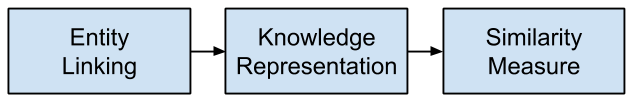
\includegraphics[width=0.95\columnwidth]{ch05_similarity/pics/methodology.png}}}
\caption{Workflow of the proposed method.}
\label{fig:methodology}
\end{figure}

\subsection{Entity Linking} %Luis
%
Entity linking is the task to associate, for a given candidate textual fragment, the most suitable entry in a reference Knowledge Base (KB) \cite{Moroetal2014b}. It encompasses similar subtasks such as Named Entity Disambiguation \cite{BunescuandPasca2006}, which is precisely linking mentions to entities to a KB, or Wikification \cite{MihalceaandCsomai2007}, specifically using Wikipedia as KB.

We considered several state-of-the-art entity linking tools, including Babelfy \cite{Moroetal2014b}, TagMe \cite{Ferraginaetal2010}, Agdistis \cite{Usbecketal2014} and DBPedia Spotlight \cite{Mendes2011}. However we opted to use the first one for consistency purposes, as in a later step we exploit \textit{SensEmbed}~\cite{Iacobaccietal2015}, a vector space representation of concepts based on BabelNet \cite{Navigli2010}. Moreover, the use of a single tool across approaches guarantees that the evaluation will only reflect the appropriateness of each one of them, and in case of error propagation all the approaches will be affected the same.

Babelfy \cite{Moroetal2014b} is a state-of-the-art system for entity linking and word sense disambiguation based on non-strict identification of candidate meanings (i.e. not necessarily exact string matching), together with a graph based algorithm that traverses the BabelNet graph and selects the most appropriate semantic interpretation for each candidate.

\subsection{Knowledge representation}\label{sec:knowledge_representations}

\subsubsection{Relation graph}\label{sec:rel_graph} %Moha

Relation extraction has been defined as the process of identifying and annotating relevant semantic relations between entities in text \cite{JiangZhai2007}. In order to exploit the semantic relations between entities present in artist biographies, we applied the method defined in \cite{Oramas2015} for relation extraction in the music domain. The method basically consists of three steps. First, entities are identified in the text by applying entity linking. Second, relations between pairs of entities occurring in the same sentence are identified and filtered by analyzing the structure of the sentence, which is obtained by running a syntactic parser based on the formalism of dependency grammar~\cite{Bohnet2010}. Finally, the identified entities and relations are modeled as a knowledge graph.
%connects pairs of entities via labeled relations.
This kind of extracted knowledge graphs may be useful for music recommendation \cite{Sordo2015}, as recommendations can be conveyed to users by means of natural language. We apply this methodology to the problem of artist similarity, by creating a graph that connects the entities detected in every artist biography. We call this approach RG (relation graph). Figure~\ref{fig:relation} shows the output of this process for a single sentence.
%Thus, two artists may be related through different paths of entities, and with different path lengths.

\begin{figure}[!htp]
\centerline{
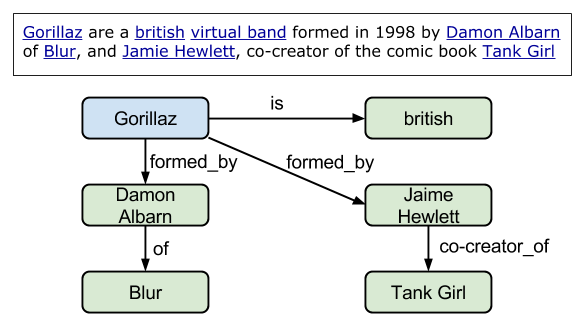
\includegraphics[width=0.95\columnwidth]{ch05_similarity/pics/RelationGraph.png}}
\caption{Relation graph of a single sentence}
\label{fig:relation}
\end{figure}


\subsubsection{Semantically enriched graph}\label{sec:semantic_enriched_graph} %Sergio

A second approach is proposed using the same set of linked entities. However, instead of exploiting natural language text, we use semantic information from the referenced knowledge base to enrich the semantics of the linked entities. We follow a semantic enrichment process similar to the one described in \cite{Ostuni2015}. We use semantic information coming from DBpedia\footnote{\url{http://dbpedia.org}}. DBpedia resources are generally classified using the DBpedia Ontology, which is a shallow, cross-domain ontology based on the most common infoboxes of Wikipedia. DBpedia resources are categorized using this ontology among others (e.g. Yago, schema.org) through the \texttt{rdfs:type} property. In addition, each Wikipedia page may be associated with a set of Wikipedia categories, which link articles under a common topic. DBpedia resources are related to Wikipedia categories through the property \texttt{dcterms:subject}.

We take advantage of these two properties to build our semantically enriched graph.
We consider three types of nodes for this graph: 1) 	artist entities obtained by matching the artist names to their corresponding DBPedia entry; 2) named entities detected by the entity linking step; and 3) Wikipedia categories associated to all the previous entities.
Edges are then added between artist entities and the named entities detected in their biographies, and between entities and their corresponding Wikipedia categories.
For the construction of the graph, we can select all the detected named entities, or we can filter them out according to the information related to their \texttt{rdfs:type} property. A set of six types was selected, including \textit{artist}, \textit{band}, \textit{work}, \textit{album}, \textit{musicgenre}, and \textit{person}, which we consider more appropriate to semantically define a musical artist.

From the previous description, we define five variants of this approach. The first variant, which we call AEC (Artists-Entities-Categories), considers all 3 types of nodes along with their relations (as depicted in Figure~\ref{fig:enriched}). The second variant, named AE (Artists-Entities) ignores the categories of the entities. The third and fourth variant, named AEC-FT and AE-FT, are similar to the first and second variant, respectively, except that the named entities are filtered using the above mentioned list of 6 entity types. Finally, the fifth variant, EC, ignores the artist entities of node type 1.

\begin{figure}[!htp]
\centerline{
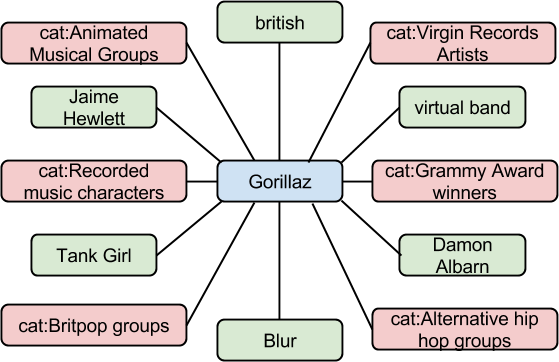
\includegraphics[width=0.95\columnwidth]{ch05_similarity/pics/EnrichedGraph1.png}}
\caption{Semantically enriched subgraph of the same sentence from Figure~\ref{fig:relation}, variant AEC with h=1}
\label{fig:enriched}
\end{figure}

%First, artist entities are added to the graph as nodes. For every artist, all entities detected in its biography are added to the graph as nodes, and connected through an edge to the artist entity. For every added entity, its associated Wikipedia categories are retrieved and added to the graph as nodes. Every entity is attached to its associated categories though and edge. Thus, a graph of artists, linked entities and semantic categories is finally generated.
%
%A second version of the graph is proposed. Instead of adding all detected entities, we filter them out according to the information related to their \texttt{rdfs:type} property. A set of six types was selected, including \textit{artist}, \textit{band}, \textit{work}, \textit{album}, \textit{musicgenre}, and \textit{person}. These types address to the entities that we consider more appropriate to semantically define a musical artist. Hence, a filtered version of the graph is built by selecting entities only of the specified types, and their corresponding categories.
%
%For evaluation purposes, we created two more versions of the graph. Both versions follow the same graph creation process, but ignoring the last step of adding categories. Though, the graphs includes only artist entities and detected entities. One version includes all detected entities, and the other only entities of the specified types.

\subsubsection{Sense embeddings}\label{sec:sense_embeddings}
The semantic representation used in this approach is based on SensEmbed \cite{Iacobaccietal2015}. SensEmbed is a vector space semantic representation of words similar to word2vec \cite{Mikolovetal2013},
%with the aggregated value than instead of plain text words,
where each vector represents a BabelNet synset and its lexicalization. Let $A$ be the set of artist biographies in our dataset. Each artist biography $a \in A$ is converted to a set of disambiguated concepts $\text{Bfy}_{a}$ after running Babelfy over it.

\subsection{Similarity approaches}

\subsubsection{SimRank} %Moha

SimRank is a similarity measure based on an simple graph-theoretic model \cite{jeh2002simrank}. The intuition is that two nodes are similar if they are referenced by similar nodes. In particular we use the definition of bipartite SimRank \cite{jeh2002simrank}. We build a bipartite graph with named entities and their corresponding Wikipedia categories (the EC variant from Section~\ref{sec:semantic_enriched_graph}). The similarity between two named entities (say $p$ and $q$) is computed with the following recursive equation:

\begin{equation}
s(p,q) = \frac{C}{|O(p)||O(q)|} \sum_{i=1}^{|O(p)|} \sum_{j=1}^{|O(q)|} s(O_i(p), O_j(q))
\end{equation}

where $O$ denotes the out-neighboring nodes of a given node and $C$ is a constant between 0 and 1. For $p = q$, $s(p,q)$ is automatically set up to $1$.
Once the similarity between all pairs of entities is obtained, we proceed to calculate the similarity between pairs of artists (say $a$ and $b$) by aggregating the similarities between the named entities identified in their biographies, as shown in the following formula:

\begin{equation}
\footnotesize
sim(a,b) = Q(a,b) \frac{1}{N} \sum_{e_a \in a} \sum_{e_b \in b} s(e_a, e_b)\quad \text{if}\ s(e_a, e_b) \geq 0.1
\end{equation}

where $s$ denotes the SimRank of entities $e_a$ and $e_b$ and $N$ is the number of ($e_a$, $e_b$) pairs with $s(e_a, e_b) \geq 0.1$. This is done to filter out less similar pairs.
%We only consider pairs of entities with $s(e_a, e_b) \geq 0.1$. This is done to filter out less similar pairs.
%
Finally, $Q(a,b)$ is a normalizing factor that accounts for the pairs of artists with more similar entity pairs than others.
%, and it is computed as follows:

%\begin{equation}
%Q(a,b) = \frac{N(a,b)^{\alpha-1}}{max\_N(a)^{\alpha}}
%\end{equation}
%
%where $N(a,b)$ is the number of ($e_a$, $e_b$) pairs with $s(e_a, e_b) \geq 0.1$, and $max\_N(a)$ is the largest value of $N$ for artist $a$.
%$\alpha$ is a parameter between 0 and 1. We empirically set $\alpha = 0.6$.


\subsubsection{Maximal common subgraph}\label{sec:method:sim:mcs} %Sergio

Maximal common subgraph (MCS) is a common distance measure on graphs. It is based on the maximal common subgraph of two graphs. MCS is a symmetric distance metric, thus $d(A,B)=d(B,A)$. It takes structure as well as content into account. According to \cite{Bunke1998}, the distance between two non empty graphs $G_{1}$ and $G_{2}$ is defined as

\begin{equation}
d(G_{1},G_{2}) = 1 - \cfrac{| mcs(G_{1},G_{2}) |}{max(|G_{1}|,|G_{2}|)}
\end{equation}

It can also be seen as a similarity measure $s$, assuming that $s=1-d$, as applied in \cite{Lux2005}. To compute this similarity measure we need to have a graph for each artist. This can be achieved by finding subgraphs in the graph approaches defined in Section~\ref{sec:knowledge_representations}. A subgraph will include an artist entity node and its neighboring nodes.
Furthermore, we apply the notion of h-hop item neighborhood graph defined in \cite{ODMD14a} to a semantic graph. Let $G=(E,P)$ be an undirected graph where $E$ represent the nodes (entities), and $P$ the set of edges with $P \subseteq E \times E$. For an artist item $a$ in $G$, its h-hop neighborhood subgraph $G^{h}(a)=(E^{h}(a),P^{h}(a))$ is the subgraph of $G$ formed by the set of entities that are reachable from $a$ in at most h hops, according to the shortest path. %An example of a 2-hop item neighborhood graph of an artist is shown in ~Fig.
Following this approach, we obtain an h-hop item neighborhood graph for each artist node of the semantic graph. Then, maximal common subgraph is computed between each pair of h-hop item neighborhood graphs. For each artist, the list of all similar artists ordered from the most similar to the less one is finally obtained.

\subsubsection{Cumulative cosine similarity} %Luis

%The semantic representation used in this approach is based on SensEmbed \cite{Iacobaccietal2015}, a vector space semantic representation of words similar to word2vec \cite{Mikolovetal2013}, with the aggregated value than instead of plain text words, each vector represents a BabelNet synset and its lexicalization. Specifically, the following steps are performed: (1) Let $A$ be the set of artist biographies in our dataset, in which each artist biography $a \in A$ is converted to a set of disambiguated concepts $\text{Bfy}_{a}$ after running Babelfy over it. (2)
For each pair of concepts $c \in \text{Bfy}_{a}$ and $c^{\prime} \in \text{Bfy}^{\prime}_{a}$ (as defined in Section \ref{sec:sense_embeddings}), we are interested in obtaining the similarity of their closest senses. This is achieved by first deriving the set of associated vectors $V_c$ and $V_{c^{\prime}}^{\prime}$ for each pair of concepts $c,\,c^{\prime}$, and then optimizing

\begin{equation}
\operatorname{max}_{v_c \in V_c , v_{c^{\prime}}^{\prime} \in V_{c^{\prime}}^{\prime}}
\left( \frac{v_c \times v_{c^{\prime}}^{\prime}}{\left\vert\left\vert{v_c}\right\vert\right\vert \left\vert\left\vert{v_{c^{\prime}}^{\prime}}\right\vert\right\vert } \right)
\end{equation}

i.e. computing cosine similarity between all possible senses (each sense represented as a vector) in an all-against-all fashion and keeping the highest scoring similarity score for each pair. Finally, the semantic similarity between two artist biographies is simply the average among all the cosine similarities between each concept pair.

\section{Experimental Setup}
\label{sec:experimentalsetup}

To evaluate the accuracy of the proposed approaches we designed an experimental evaluation over two datasets. The first dataset contains 2,336 artists and it is evaluated using the list of similar artists provided by the Last.fm API as a ground truth. The second dataset contains 188 artists, and it is evaluated against user similarity judgements from the MIREX Audio Music Similarity and Retrieval task.
%More information, as well as data, can be accessed online at http://music-ir.org/mirex/wiki/MIREX\_HOME} Audio and Music Similarity evaluation dataset.
Apart from the defined approaches, a pure text-based approach for document similarity is added to act as a reference for the obtained results.

\subsection{Datasets}

\subsubsection{Last.fm dataset}\label{sec:lastfm_dataset}

A dataset of 2,336 artist biographies was gathered from Last.fm. The artists in this dataset share a set of restrictions.
Their biography has at least 500 characters and is written in English.
All of the artists have a correspondent Wikipedia page, and we have been able to mapped it automatically, obtaining the DBpedia URI of every artist.
For every artist, we queried the getSimilar method of the Last.fm API and obtained an ordered list of similar artists. Every artist in the dataset fulfills the requirement of having at least 10 similar artists within the dataset.
We used these lists of similar artists as the ground truth for our evaluation.
%As the list contains at least 10 similar artists within the dataset, we can evaluate top-10 similarity.

\subsubsection{MIREX dataset} %Moha

To build this dataset, the gathered artists from Last.fm
%(without the application of the last restriction mentioned in Section~\ref{sec:lastfm_dataset})
were mapped to the MIREX Audio Music Similarity task dataset. The AMS dataset (7,000 songs from 602 unique artists) contains human judgments of song similarity. According to~\cite{Schedl2013}, the similarity between two artists can be roughly estimated as the average similarity between their songs. We used the same approach in~\cite{Schedl2013}, that is, two artists were considered similar if the average similarity score between their songs was at least 25 (on a fine scale between 0 and 100).

%to use this dataset for artist similarity evaluation.
After the mapping, we obtained an overlap of 268 artists.
%We used this dataset of 268 artists to compute similarity using the different approaches.
As we want to evaluate Top-10 similarity, every artist in the ground truth dataset should have information of at least 10 similar artists. However, not every artist in the MIREX evaluation dataset fulfills this requirement. Therefore, after removing the artists with less than 10 similars, we obtained a final dataset of 188 artists, and used it for the evaluation.

\subsection{Baseline} %Moha
In order to assess the goodness of our approaches, we need to define a baseline approach with which to compare to. The baseline used in this paper is a classic vector-based model approach used in many Information Retrieval systems. A text document is represented as a vector of word frequencies (after removing English stopwords and words with less than 2 characters), and a matrix is formed by aggregating all the vectors. The word frequencies in the matrix are then re-weighted using TF-IDF, and finally latent semantic analysis (LSA) \cite{Deerwesteretal1990} is used to produce a vector of concepts for each document. The similarity between two documents can be obtained by using a cosine similarity over their corresponding vectors.

\begin{table}[ht!]
\small
\centering
	\begin{tabular}{  lllll }
 	\toprule
& \multicolumn{2}{c}{Precision@N} & \multicolumn{2}{c}{nDCG@N} \\
\cmidrule(lr){2-3}
\cmidrule(lr){4-5}
	Approach variants & N=5 & N=10 & N=5 & N=10 \\
	\midrule
LSA & 0.100 & 0.169 & 0.496 & 0.526 \\
RG MCS 1-hop & 0.059 & 0.087 & 0.465 & 0.476 \\
RG MCS 2-hop & 0.056 & 0.101 & 0.433 & 0.468 \\
AE MCS & 0.106 & 0.178 & 0.503  & 0.517 \\
AE-FT MCS & 0.123 & 0.183 & 0.552 & 0.562 \\
AEC MCS 1-hop & 0.120 & 0.209 & 0.573 & 0.562 \\
AEC MCS 2-hop & 0.086 & 0.160 & 0.550 & 0.539 \\
AEC-FT MCS 1-hop & \textbf{0.140} & \textbf{0.218} & \textbf{0.588} & \textbf{0.578} \\
AEC-FT MCS 2-hop & 0.100 & 0.160 & 0.527 & 0.534 \\
EC SimRank & 0.097& 0.171 &  0.509 & 0.534 \\
SE Cosine & 0.095 & 0.163 & 0.454 & 0.484 \\
\bottomrule	
	\end{tabular}
	\caption{Precision and normalized discounted cumulative gain for Top-N artist similarity using the MIREX dataset (N=\{5, 10\})}	
	\label{tbl:res_mirex}
\end{table}

\begin{table}
\small
\centering
	\begin{tabular}{ lllll }
 	\toprule
	& \multicolumn{2}{c}{Precision@N} & \multicolumn{2}{c}{nDCG@N} \\
\cmidrule(lr){2-3}
 \cmidrule(lr){4-5}
	Approach variants & N=5 & N=10 & N=5 & N=10 \\
	\midrule
LSA & 0.090 & 0.088 & 0.233 & 0.269 \\
RG MCS 1-hop & 0.055 & 0.083 & 0.126 & 0.149 \\
AE MCS & 0.124 & 0.200 & 0.184 & 0.216 \\
AE-FT MCS & 0.136 & 0.201 & 0.224 & 0.260 \\
AEC MCS 1-hop & 0.152 & 0.224 & 0.277 & 0.297 \\
AEC-FT MCS 1-hop & \textbf{0.160} & \textbf{0.242} & \textbf{0.288} & \textbf{0.317} \\
\bottomrule
	\end{tabular}
	\caption{Precision and normalized discounted cumulative gain for Top-N artist similarity using the Last.fm dataset (N=\{5, 10\})}	
	\label{tbl:res_lastfm}
\end{table}
\subsection{Evaluated approaches}\label{sec:eval_approaches} %Sergio

From all possible combinations of knowledge representations, similarity measures and parameters, we selected a set of 10 different approach variants. The prefixes AEC, RG and AE refer to the graph representations (see Sections \ref{sec:rel_graph} and \ref{sec:semantic_enriched_graph}). %AEC refers to the artist entity categories graph, RG to the graph of relations extracted from text, and AE to a graph with artist entities and named entities.
SE refers to the sense embeddings approach, and LSA to the latent semantic analysis baseline approach. When these prefixes are followed by FT, it means that the entities in the graph have been filtered by type. The second term in the name refers to the similarity measure. MCS refers to maximal common subgraph, and SimRank and Cosine to SimRank and cumulative cosine similarity measures. MCS approaches are further followed by a number indicating the number of h-hops of the neighborhood subgraph.


\begin{table*}[ht!]
\centering
	\begin{tabular}{ lllllllll }
 	\toprule
& \multicolumn{8}{c}{Genres} \\
\cmidrule(lr){2-9}
	Approach variants & Blues & Country & Edance & Jazz & Metal & Rap & Rocknroll & Overall\\
	\midrule
Ground Truth & 5.78 & 5.46 & 6.88 & 7.04 & 7.10 & 8.68 & 5.17 & 6.53\\
\midrule[.2pt]
LSA & 4.43 & 4.12 & 3.80 & 4.64 & 5.79 & 5.08 & 4.74 & 4.69\\
RG MCS 1-hop & 2.63 & 3.50 & 1.50 & 2.95 & 4.00 & 2.54 & 1.70 &  2.68\\
RG MCS 2-hop & 4.14 & 4.92 & 1.69 & 2.80 & 3.78 & 3.06 & 2.77 & 3.27\\
AE MCS & 5.52 & 5.15 & 4.36 & 7.00 & 4.34 & 5.36 & 4.46 & 5.11\\
AE-FT MCS & 5.43 & 6.12 & 4.16 & 6.20 & 6.32 & 5.36 & 3.77 & 5.26 \\
AEC MCS 1-hop & \textbf{7.22} & 5.92 & 5.24 & 7.12 & 5.48 & 6.92 & 4.86 & 6.02 \\
AEC MCS 2-hop & 4.22 & 3.69 & 4.56 & 6.20 & 4.55 & 4.64 & 4.09 & 4.54 \\
AEC-FT MCS 1-hop & 6.91 & \textbf{6.80} & \textbf{6.04} & \textbf{7.60} & \textbf{6.79} & \textbf{7.12} & \textbf{5.37} & \textbf{6.59} \\
AEC-FT MCS 2-hop & 4.09 & 4.36 & 5.56 & 6.72 & 4.39 & 4.16 & 3.77 & 4.67 \\
EC SimRank & 6.74 & 5.38 & 3.16 & 6.40 & 4.59 & 4.44 & 3.80 & 4.85 \\
SE Cosine & 3.39 & 5.50 & 5.32 & 5.16 & 4.31 & 5.36 & 4.31 & 4.75 \\
\bottomrule	
	\end{tabular}
	\caption{Average genre distribution of the top-10 similar artists using the MIREX dataset. In other words, on average, how many of the top-10 similar artists are from the same genre as the query artist. LSA stands for Latent Semantic Analysis, RG for Relation Graph, SE for Sense Embeddings,  and AE, AEC and EC represent the semantically enriched graphs with Artists-Entities, Artist-Entities-Categories, and Entities-Categories nodes, respectively. As for the similarity approaches, MCS stands for Maximum Common Subgraph.}	
	\label{tbl:res_genre_distrib}
\end{table*}


%\begin{table*}[ht!]
%\small
%\centering
%	\begin{tabular}{ lllllllll }
%  	\toprule
% & \multicolumn{8}{c}{Genres} \\
% \cmidrule(lr){2-9}
%	Approach variants & Blues & Country & Edance & Jazz & Metal & Rap & Rocknroll & Overall\\
%	\midrule
%Grount Truth & 5.78\scalebox{0.8}{$\pm2.62$} & 5.46\scalebox{0.8}{$\pm1.89$} & 6.88\scalebox{0.8}{$\pm2.14$} & 7.04\scalebox{0.8}{$\pm1.84$} & 7.10\scalebox{0.8}{$\pm1.67$} & 8.68\scalebox{0.8}{$\pm1.09$} & 5.17\scalebox{0.8}{$\pm1.36$} & 6.53\scalebox{0.8}{$\pm2.15$}\\
%\midrule[.2pt]
%LSA & 4.43\scalebox{0.8}{$\pm2.00$} & 4.12\scalebox{0.8}{$\pm2.58$} & 3.80\scalebox{0.8}{$\pm1.67$} & 4.64\scalebox{0.8}{$\pm2.56$} & 5.79\scalebox{0.8}{$\pm2.28$} & 5.08\scalebox{0.8}{$\pm2.31$} & 4.74\scalebox{0.8}{$\pm2.03$} & 4.69\scalebox{0.8}{$\pm2.30$}\\
%RG MCS 1-hop & 2.63\scalebox{0.8}{$\pm2.87$} & 3.50\scalebox{0.8}{$\pm2.53$} & 1.50\scalebox{0.8}{$\pm0.98$} & 2.95\scalebox{0.8}{$\pm1.64$} & 4.00\scalebox{0.8}{$\pm2.24$} & 2.54\scalebox{0.8}{$\pm1.87$} & 1.70\scalebox{0.8}{$\pm1.51$} &  2.68\scalebox{0.8}{$\pm2.20$}\\
%RG MCS 2-hop & 4.14\scalebox{0.8}{$\pm2.61$} & 4.92\scalebox{0.8}{$\pm2.30$} & 1.69\scalebox{0.8}{$\pm1.26$} & 2.80\scalebox{0.8}{$\pm1.57$} & 3.78\scalebox{0.8}{$\pm2.22$} & 3.06\scalebox{0.8}{$\pm2.16$} & 2.77\scalebox{0.8}{$\pm1.60$} & 3.27\scalebox{0.8}{$\pm2.18$}\\
%AE MCS & 5.52\scalebox{0.8}{$\pm2.57$} & 5.15\scalebox{0.8}{$\pm2.80$} & 4.36\scalebox{0.8}{$\pm1.94$} & 7.00\scalebox{0.8}{$\pm2.77$} & 4.34\scalebox{0.8}{$\pm1.58$} & 5.36\scalebox{0.8}{$\pm2.48$} & 4.46\scalebox{0.8}{$\pm1.86$} & 5.11\scalebox{0.8}{$\pm2.45$}\\
%AE-FT MCS & 5.43\scalebox{0.8}{$\pm2.86$} & 6.12\scalebox{0.8}{$\pm2.65$} & 4.16\scalebox{0.8}{$\pm2.01$} & 6.20\scalebox{0.8}{$\pm2.84$} & 6.32\scalebox{0.8}{$\pm2.75$} & 5.36\scalebox{0.8}{$\pm2.73$} & 3.77\scalebox{0.8}{$\pm1.85$} & 5.26\scalebox{0.8}{$\pm2.71$} \\
%AEC MCS 1-hop & \textbf{7.22}\scalebox{0.8}{$\pm2.90$} & 5.92\scalebox{0.8}{$\pm2.72$} & 5.24\scalebox{0.8}{$\pm2.21$} & 7.12\scalebox{0.8}{$\pm2.73$} & 5.48\scalebox{0.8}{$\pm1.87$} & 6.92\scalebox{0.8}{$\pm2.88$} & 4.86\scalebox{0.8}{$\pm1.50$} & 6.02\scalebox{0.8}{$\pm2.57$} \\
%AEC MCS 2-hop & 4.22\scalebox{0.8}{$\pm2.81$} & 3.69\scalebox{0.8}{$\pm2.45$} & 4.56\scalebox{0.8}{$\pm2.26$} & 6.20\scalebox{0.8}{$\pm3.22$} & 4.55\scalebox{0.8}{$\pm2.50$} & 4.64\scalebox{0.8}{$\pm2.59$} & 4.09\scalebox{0.8}{$\pm1.56$} & 4.54\scalebox{0.8}{$\pm2.59$} \\
%AEC-FT MCS 1-hop & 6.91\scalebox{0.8}{$\pm3.74$} & \textbf{6.80}\scalebox{0.8}{$\pm2.15$} & \textbf{6.04}\scalebox{0.8}{$\pm1.87$} & \textbf{7.60}\scalebox{0.8}{$\pm2.38$} & \textbf{6.79}\scalebox{0.8}{$\pm2.14$} & \textbf{7.12}\scalebox{0.8}{$\pm2.86$} & \textbf{5.37}\scalebox{0.8}{$\pm1.57$} & \textbf{6.59}\scalebox{0.8}{$\pm2.52$} \\
%AEC-FT MCS 2-hop & 4.09\scalebox{0.8}{$\pm2.76$} & 4.36\scalebox{0.8}{$\pm2.24$} & 5.56\scalebox{0.8}{$\pm3.16$} & 6.72\scalebox{0.8}{$\pm2.89$} & 4.39\scalebox{0.8}{$\pm1.97$} & 4.16\scalebox{0.8}{$\pm2.52$} & 3.77\scalebox{0.8}{$\pm1.17$} & 4.67\scalebox{0.8}{$\pm2.59$} \\
%EC SimRank & 6.74\scalebox{0.8}{$\pm2.19$} & 5.38\scalebox{0.8}{$\pm3.03$} & 3.16\scalebox{0.8}{$\pm1.49$} & 6.40\scalebox{0.8}{$\pm2.62$} & 4.59\scalebox{0.8}{$\pm1.63$} & 4.44\scalebox{0.8}{$\pm1.86$} & 3.80\scalebox{0.8}{$\pm1.85$} & 4.85\scalebox{0.8}{$\pm2.45$} \\
%SE Cosine & 3.39\scalebox{0.8}{$\pm1.97$} & 5.50\scalebox{0.8}{$\pm2.15$} & 5.32\scalebox{0.8}{$\pm1.85$} & 5.16\scalebox{0.8}{$\pm2.31$} & 4.31\scalebox{0.8}{$\pm1.29$} & 5.36\scalebox{0.8}{$\pm2.51$} & 4.31\scalebox{0.8}{$\pm1.85$} & 4.75\scalebox{0.8}{$\pm2.12$} \\
%\bottomrule	
%	\end{tabular}
%	\caption{Genre distribution of the top-10 similar artists using the MIREX dataset}	
%	\label{tbl:res_genre_distrib}
%\end{table*}

\subsection{Evaluation measures}

To measure the accuracy of the artist similarity we adopt two standard performance metrics such as Precision@N, and nDCG@N (normalized discounted cumulative gain).
%We applied the metrics as defined in \cite{Steck13} for evaluating recommendation, but adapted to the problem of artist similarity.
Precision@N is computed as the number of relevant items (i.e., true positives) among the top-N items divided by $N$, when compared to a ground truth.
%A relevant item is an item in the list of $N$ similar artists suggested by the system for an artist $a$, that is also in the ground truth list of N similar artists of the same artist $a$.
%Recall@N (R@N) is computed as the ratio between the number of relevant items among the top-N items and the number items in the ground truth list.
Precision considers only the relevance of items, whilst nDCG takes into account both relevance and rank position. Denoting with  $s_{ak}$ the relevance of the item in position $k$ in the Top-N list for the artist $a$, then nDCG@N for $a$ can be defined as:
%%%%%%%%%%%%%%%%%%%%%%%%%%%
\begin{equation}\label{eq:recall}
\text{nDCG@N} = \frac{1 }{\text{IDCG@N}} \sum^N_{k=1} \frac{ 2^{ s_{ak}} -1 }{\log_2 (1+k)}
\end{equation}
%%%%%%%%%%%%%%%%%%%%%%%%%%%
where IDCG@N indicates the score obtained by an ideal or perfect Top-N ranking and acts as a normalization factor. We run our experiments for $N=5$ and $N=10$.
%In Tables~\ref{tbl:res_mirex} and~\ref{tbl:res_lastfm} average values of P@N and nDCG@N among all the evaluated artists are shown.

\section{Results and discussion} %Sergio
\label{sec:results}
We evaluated all the approach variants described in Section~\ref{sec:eval_approaches} on the MIREX dataset, but only a subset of them on the Last.fm dataset, due to the high computational cost of some of the approaches.
%We initially worked on the MIREX dataset, as the number of artists was smaller and the computation of the algorithms was much faster. However, to ensure the credibility of the results, we applied some of the approach variants in a bigger dataset.

Table~\ref{tbl:res_mirex} shows the Precision@N and nDCG@N results of the evaluated approaches using the MIREX dataset, while Table~\ref{tbl:res_lastfm} shows the same results for the Last.fm dataset. We obtained very similar results in both datasets. The approach that gets best performance for every metric, dataset and value of N is the combination of the Artists-Entities-Categories graph filtered by types, with the maximal common subgraph similarity measure using a value of $h=1$ for obtaining the h-hop item neighborhood graphs.

Furthermore, given that the MIREX AMS dataset also provides genre data, we analyzed the distribution of genres in the top-10 similar artists for each artist, and averaged them by genres. The idea is that an artist's most similar artists should be from the same genre as the seed artist.
Table~\ref{tbl:res_genre_distrib} presents the results. Again, the best results are obtained with the approach that combines the Artists-Entities-Categories graph filtered by types, with the maximal common subgraph similarity measure using a value of $h=1$ for the h-hop item neighborhood graphs.

We extract some insights from these results. First, semantic approaches are able to improve pure text-based approaches. Second, using knowledge from an external knowledge base provides better results than exploiting the relations inside the text. Third, using a similarity measure that exploits the structure and content of a graph, such as maximal common subgraph, overcomes other similarity measures based on semantic similarity among entity mentions in document pairs.

%\begin{table*}
%\centering
%	\begin{tabular}{  lllllll }
%    	\toprule
%	& \multicolumn{3}{c}{N=5} & \multicolumn{3}{c}{N=10} \\
%	\cmidrule(lr){2-4}
%	\cmidrule(lr){5-7}
%	Approach variants & P@N & R@N & nDCG@N & P@N & R@N & nDCG@N \\
%	\midrule
%LSA& 0.100 & 0.025 & 0.496 & 0.169 & 0.081 & 0.526 \\
%RG MCS 1-hop& 0.059 & 0.013 & 0.465 & 0.087 & 0.039 & 0.476 \\
%RG MCS 2-hop& 0.056 & 0.012 & 0.433 & 0.101 & 0.049 & 0.468 \\
%ENT MCS 1-hop& 0.106 & 0.026 & 0.503 & 0.178 & 0.087 & 0.517 \\
%ENT-FT MCS 1-hop& 0.123 & 0.029 & 0.552 & 0.183 & 0.091 & 0.562 \\
%EC MCS 1-hop& 0.120 & 0.030 & 0.573 & 0.209 & 0.105 & 0.562 \\
%EC MCS 2-hop& 0.086 & 0.021 & 0.550 & 0.160 & 0.075 & 0.539 \\
%EC-FT MCS 1-hop& \textbf{0.140} & \textbf{0.034} & \textbf{0.588} & \textbf{0.218} & \textbf{0.110} & \textbf{0.578} \\
%EC-FT MCS 2-hop& 0.100 & 0.023 & 0.527 & 0.160 & 0.078 & 0.534 \\
%EC SimRank& 0.097 & 0.025 & 0.509 & 0.171 & 0.086 & 0.534 \\
%SE Cosine& 0.095 & 0.023 & 0.454 & 0.163 & 0.080 & 0.484 \\
%\bottomrule	
%  	\end{tabular}
%	\caption{Precision, Recall and nNDCG for Top-N artist similarity in MIREX dataset}	
%	\label{tbl:res_mirex}
%\end{table*}




%\begin{table*}
%\centering
%	\begin{tabular}{ | l | c | c | c | c | c | c | }
%    	\hline
%	& \multicolumn{3}{|c|}{N=5} & \multicolumn{3}{|c|}{N=10} \\
%	\hline
%	Approach variants & P@N & R@N & nDCG@N & P@N & R@N & nDCG@N \\
%	\hline
%LSA& 0.090 & 0.022 & 0.233 & 0.088 & 0.046 & 0.269 \\
%RG MCS 1-hop& 0.055 & 0.013 & 0.126 & 0.083 & 0.039 & 0.149 \\
%ENT MCS 1-hop& 0.124 & 0.032 & 0.184 & 0.200 & 0.104 & 0.216 \\
%ENT-FT MCS 1-hop& 0.136 & 0.036 & 0.224 & 0.201 & 0.101 & 0.260 \\
%EC MCS 1-hop& 0.152 & 0.039 & 0.277 & 0.224 & 0.117 & 0.297 \\
%EC-FT MCS 1-hop& \textbf{0.160} & \textbf{0.041} & \textbf{0.288} & \textbf{0.242} & \textbf{0.123} & \textbf{0.317} \\
%\hline	
%  	\end{tabular}
%	\caption{Precision, Recall and nNDCG for Top-N artist similarity in Last.fm dataset}	
%	\label{tbl:res_lastfm}
%\end{table*}

\section{Conclusion} %Todos
\label{sec:conclusion}

In this paper we presented a methodology that exploits semantic technologies for computing artist similarity, which can be divided in three main steps: First, named entity mentions are identified in the text and linked to a knowledge base. Then, these entity mentions are used to construct a semantically motivated knowledge representation.
%, in the form of a semantic graph or a mapping to a vector-space model.
Finally a similarity function is defined on top of the knowledge representation to compute the similarity between artists.
For each one of these steps we explored several approaches, and evaluated them against a small dataset of 188 artist biographies, and a larger dataset of 2,336 artists, both obtained from Last.fm.
%The former dataset was mapped to the MIREX Audio and Music Similarity evaluation dataset, so that its similarity judgments can be used as ground truth. For the latter dataset we used the similarity between artists as provided by the Last.fm API. We used Precision@$N$ and nDCG@$N$ as our evaluation measures, with $N=\{5, 10\}$. Furthermore, we also analyzed the distribution of genres of top-N artist similarity, with $N=10$.

Results showed that a combination of the Artists-Entity-Categories graph filtered by types, and a maximal common subgraph similarity measure using a value of $h=1$ for obtaining the h-hop item neighborhood graphs, clearly outperforms a baseline approach that exploits word co--occurrences and latent factors. In the light of these results, the following conclusions can be drawn: First, semantic approaches may outperform pure text-based approaches. Second, we observe that knowledge leveraged from external ontologies may improve the accuracy of the similarity measure. Third, reducing noise by filtering linked entities by type is a rewarding step that contributes to an improved performance. Finally, we show that similarity measures that take into consideration the structure and content of a graph representation may achieve much higher performance.
%, not only in terms of precision, but also in terms of computational cost, being the fastest approach by far.

There are still many avenues for future work. We would like to compare our semantic-based approach with acoustic and collaborative filtering approaches. In addition, the use of text sources different from artist biographies can be studied. Finally, in order to improve the results obtained by our semantic approach, different state-of-the-art entity linking tools can be applied, or a specific entity linking tool for the music domain could be created for this purpose.